%!TeX root=../tese.tex
%("dica" para o editor de texto: este arquivo é parte de um documento maior)
% para saber mais: https://tex.stackexchange.com/q/78101

\chapter{Metodologia}

Nesta seção, iremos discutir a ingestão e tratamento dos dados, bem como os métodos matemáticos de análise. 

\section{O General Transit Feed Specification (GTFS)}

Buscando padronizar os dados de transporte público para uso no Google Maps, o Google criou, em meados de 2006, em parceria com cidades dos Estados Unidos, o formato GTFS (Google Transit Feed Specification). A partir de 2010, o termo foi alterado para não ter mais relação com o Google, tornando-se General Transit Feed Specification \citep{gtfs_org_about}. 

O GTFS é um formato de organização de dados que permite que agências de transporte publiquem seus dados para uso de diversos agentes, desde empresas até estudantes e planejadores de políticas públicas, permitindo que empresas como a Google forneçam aos usuários detalhes sobre as rotas, paradas e horários das linhas de transporte.

\begin{figure}[H]
    \centering
    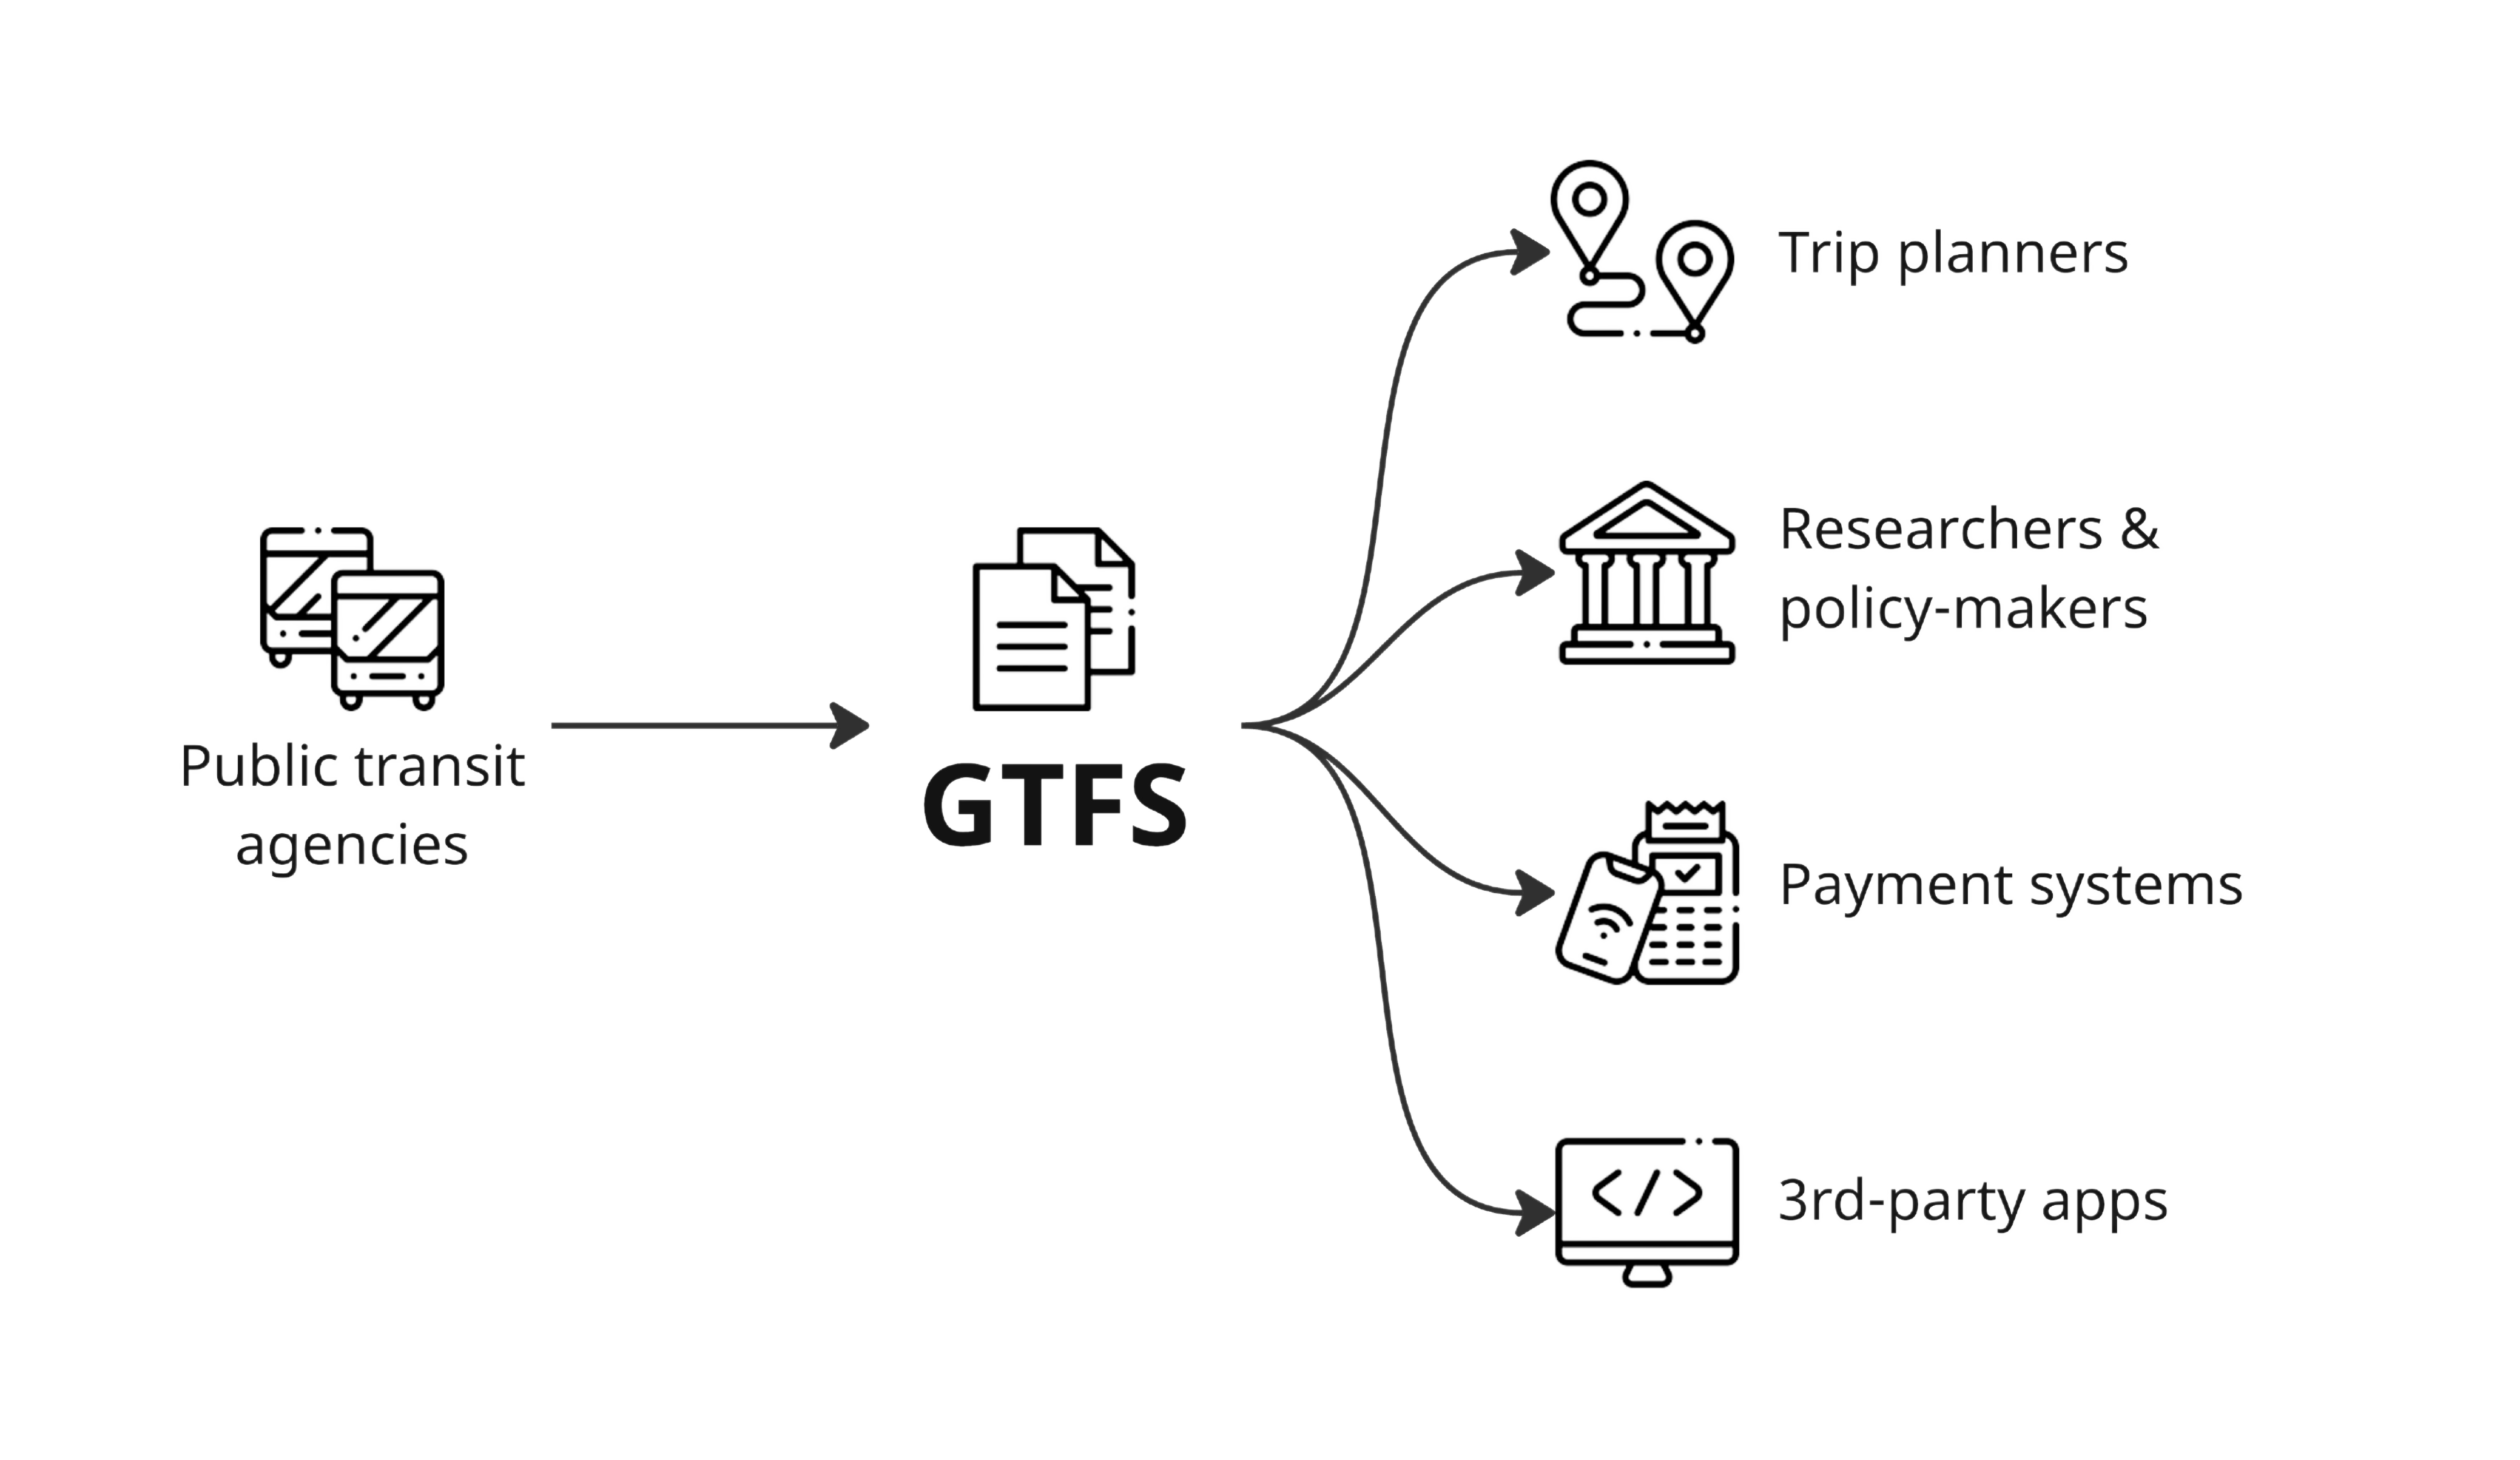
\includegraphics[width=0.8\textwidth]{figuras/organizacao gtfs.png}
    \caption{Diagrama da estrutura do GTFS. \\ Fonte: GTFS Org}
    \label{fig:minha-imagem}
\end{figure}

Nessa base de dados, podemos obter tanto dados de movimento em tempo real do transporte quanto dados dos horários e rotas programadas. Para este trabalho, utilizamos as informações de horários de paradas, paradas, viagens e rotas do GTFS fornecido pela SPTrans. Para ter acesso aos dados do GTFS, é necessário fazer download de um arquivo .zip, que contém 10 arquivos no formato csv e tipo .txt, sendo necessária autenticação no site da SPTrans, que não permite scraping tão facilmente, por conta do login. Logo, para obter os dados do GTFS, teremos que fazer download manualmente através do site da SPTrans. 

Além do GTFS, a SPTrans também disponibiliza a  API do Olho Vivo, que oferece diversos serviços que permitem o acesso em tempo real a informações sobre o transporte público da cidade de São Paulo. Os dados são disponibilizados no formato JSON e seguem uma estrutura REST, o que facilita a obtenção massiva. Com um simples cadastro, é possível gerar uma chave para uso da API, que permite acessar dados de linhas, paradas, corredores, posição dos veículos, previsão de chegada e etc. Através de requisições com a biblioteca requests do python, conseguimos obter os dados do objeto de linhas, paradas e previsão de chegada, porém, os objetos de previsão de chegada e paradas retornam apenas dados sobre paradas em corredores de ônibus, logo, a API não fornece dados sobre todas as linhas de ônibus que são operadas pela SPTrans na cidade de São Paulo, representando uma falha na disponibilização de informações por parte da SPTrans. Uma possível melhoria da API do Olho Vivo seria a disponibilização do GTFS na API REST.

Nos arquivos \verb|stop_times, stops, trips e routes,| conseguimos obter dados sobre a localização de cada parada (com as coordenadas geográficas) por linha, bem como o tipo de itinerário (sábado, domingo, DU, todos os dias), a frequência planejada dos ônibus e informações descritivas de cada linha. Após juntar todos os dados, obtemos uma tabela com as linhas, que vamos chamar de rotas, tendo 1342 valores, e uma com as viagens de cada rota, com 88534 dados. Essa será a tabela que iremos utilizar para fazer as análises iniciais. 

Na seção \ref{sec:exploracaoinicial}, descobrimos que os dados estão incompletos, o que não nos permite fazer uma análise integral das rotas, já que cada GTFS é referente apenas ao mês anterior ao qual ele foi publicado. Por conta dessa inconsistência, solicitamos dados adicionais a SPTrans, tópico que será tratado na seção \ref{sec:esic}. Por meio dessa solicitação, conseguimos obter 10 anos de histórico do GTFS.


\section{Dados de passageiros por linha}

A prefeitura de São Paulo disponibiliza em seu site, na seção de acesso à informação \footnote{\url{https://capital.sp.gov.br/web/mobilidade/w/passageiros-transportados-2025}} os dados de passageiros transportados nas linhas da capital, com granularidade diária e mensal, através de arquivos no formato xls (um formato antigo de planilhas utilizado pelo Microsoft Excel entre 97 e 2003, que ainda pode ser lido através de código ou versões modernas do Excel). Os dados são obtidos ao passar algum tipo de bilhete único na leitora dos veículos ou estações de trem e metrô. Além do total de passageiros, também há divisões entre bilhetes estudantis, gratuitos, vale comum e vale transporte, com as respectivas versões mensais: estudantil mensal, vale comum mensal, vale transporte mensal. Também há dados de pagamento feito em dinheiro, já que nesses casos, o cobrador/motorista passa o bilhete institucional para liberar a pessoa.

Através de um processo de \textit{web scraping}, realizamos o download dos dados diários disponíveis no site da SPTrans, sendo necessário o acesso a 10 páginas diferentes do site, com cada uma contendo os dados de um ano específico, de 2015 a 2025. No total, foram coletados aproximadamente 365 arquivos por ano, correspondentes a um arquivo por dia, abrangendo o período de 2015 a 2024. Além disso, foram obtidos dados de 235 dias do ano de 2025. O processo de download dos arquivos não pode ser 100\% automatizado pois os caminhos onde podemos acessar os arquivos variam, conforme exemplo:

\begin{itemize}
    \item 17 de janeiro de 2025: https://prefeitura.sp.gov.br/documents/d/mobilidade/17jan2025-1-xls
    \item 25 de abril de 2024: https://www.prefeitura.sp.gov.br/cidade/secretarias/upload/25ABR2024.xls
    
\end{itemize}

O processo de coleta foi relativamente rápido, com um tempo médio de 5 minutos para o download completo dos arquivos xls. No entanto, a unificação e padronização dos dados, que possuíam diferentes nomenclaturas e organizações, representaram uma etapa significativamente mais trabalhosa, exigindo cerca de 50 minutos para serem processados e consolidados. Optamos por juntar todos os dados em um único arquivo no formato parquet, que permite processamento paralelo eficiente e consultas rápidas, por serem estruturados em colunas e facilmente particionáveis \citep{parquet_optimization}.

Um dos problemas que encontramos nos dados é nome das linhas. Nos arquivos disponibilizados no site, cada linha é disponibilizada da forma "Código - Nome da linha", podendo haver exceções e erros ortográficos. No nosso processo, vamos descartar o nome da linha, e obter o código com um script genérico, que funciona para a maioria, mas não todos os dados. Devido ao volume, vamos definir que essa perda é aceitável.

\subsection{Padronização e otimização}

Para ler os 3737 arquivos xls baixados, gastamos 25min27s e precisamos criar condições para tratar corretamente o cabeçalho de cada planilha. A cada ano, as informações dispostas eram as mesmas, porém, apresentadas com nomenclaturas diferentes, e às vezes com notas que ocupavam as 2 ou 3 primeiras linhas do arquivo. Inicialmente, então, lemos todos os arquivos xls e convertemos todos em parquet, buscando otimizar a leitura dos dados antes de iniciar qualquer tipo de tratamento. Apesar de encontrarmos alguns erros por arquivos corrompidos, conseguimos converter 3679 (98,44\%) dos arquivos xls para parquet. A leitura dos arquivos parquet levou cerca de 46 segundos, representando uma melhoria de 3319\% no desempenho.

Para obter uma única tabela, precisávamos concatenar todos os dados obtidos, o que levou a um problema de padronização dos nomes das colunas. Juntando os dados de todos os anos, havia cerca de 40 colunas diferentes, com cerca de 3 variações para cada tipo de dados. Por exemplo, para o dado "bilhete estudante", as nomenclaturas eram:

\begin{itemize}
\item \verb|passageiros pagantes bilhete único estudante\n\n(d)|
\item \verb|passageiros pagtes estudante|
\item \verb|soma de passageiros pagantes bilhete único estudante\n\n(d)|
\end{itemize}

Acreditamos que essas diferenças ocorreram por mudanças ao longo dos anos. Para resolver esse problema, criamos um dicionário para renomear as tabelas antes de realizar a unificação.


\subsection{Unificação}

Após obtermos os 3737 DataFrames, renomeamos e concatenamos todos, o que levou 32min1s. A tabela resultante possui 25 colunas e 4.935.341 linhas, representando os dados de passageiros 2015 a 2025. 

Antes de salvar o DataFrame obtido em um arquivo parquet, vamos criar a coluna \verb|route_id| para armazenar o código da linha, que extraímos da coluna linha com uma generalização, conforme explicitado antes. Além disso, também vamos criar a coluna \verb|passageiros_integracao|, somando os dados de todas as outras integrações, e atualizar as colunas \verb|passageiros_vale_transporte, passageiros_comum e passageiros_estudante|, somando os dados mensais de cada um, além do dado \verb|passageiros_comum_vt| para o vale transporte.

Com os dados unificados, salvamos um único arquivo parquet, que, mesmo contendo 4.935.341 linhas e 25 colunas, pode ser lido em cerca de 7s.

\section{Dados complementares}


\subsection{Dados do IBGE}\label{sec:ibge}

Em 2025, o IBGE disponibilizou os dados agregados por setor censitário do censo de 2022, com informações geográficas sobre os bairros de São Paulo, além de estatísticas sobre os moradores\footnote{\url {https://www.ibge.gov.br/estatisticas/sociais/populacao/22827-censo-demografico-2022.html?edicao=41852\&t=resultados}}. Foi utilizado o formato Sistemas de Informação Geográfica (SIG), que disponibiliza os dados em formatos como shapefiles ou GeoJSONs, para representar dados geoespaciais vetoriais, como pontos, linhas e polígonos. Os setores censitários de uma metrópole como São Paulo são super fragmentados, o que permite um estudo mais aprofundado dos dados.

Para realizar a leitura e manipulação desses arquivos em Python, utilizaremos a biblioteca GeoPandas, que estende a funcionalidade do Pandas para trabalhar com dados geoespaciais de forma simples e eficiente, permitindo a leitura de arquivos com shapefiles. 

As estatísticas sobre a população obtidas foram as seguintes:

\begin{table}[H]
\centering
\begin{tabularx}{\textwidth}{|c|X|}
\hline
\textbf{Código} & \textbf{Descrição} \\
\hline
V0001 & Total de pessoas \\
V0002 & Total de Domicílios (DPPO + DPPV + DPPUO + DPIO + DCCM + DCSM) \\
V0003 & Total de Domicílios Particulares (DPPO + DPPV + DPPUO + DPIO) \\
V0004 & Total de Domicílios Coletivos (DCCM + DCSM) \\
V0005 & Média de moradores em Domicílios Particulares Ocupados (Total pessoas em Domicílios Particulares Ocupados / DPPO + DPIO) \\
V0006 & Percentual de Domicílios Particulares Ocupados Imputados (Total DPO imputados / Total DPO) \\
V0007 & Total de Domicílios Particulares Ocupados (DPPO + DPIO) \\
\hline
\end{tabularx}
\caption{Variáveis de domicílios e população. Fonte: IBGE}
\label{tab:variaveis_domicilios_populacao}
\end{table}

Para o nosso trabalho, utilizaremos predominantemente o dado "Total de pessoas" na coluna v0001. Vale notar que os dados disponibilizados pelo IBGE têm uma granularidade altíssima, sendo tabelas muito pesadas, que demandam alta quantidade de memória para realizar joins espaciais. 

Para utilizar os dados do Censo 2022, juntamos a coordenada geográfica das paradas com a coordenada geográfica de cada setor censitário, através de um spatial join de "within", que verifica se o ponto da coluna A está dentro do polígono B, para cada ponto da coluna A e cada polígono da coluna B. No nosso caso, vamos verificar se o polígono com a coordenada de uma parada está dentro do polígono de um setor censitário. Assim, cada parada passa a conter, adicionalmente, os atributos demográficos do bairro em que está inserida, como população total, número de domicílios e área territorial, além das colunas categóricas que identificam região, distrito e subprefeitura.  

O GeoPandas oferece suporte nativo para indexação espacial utilizando o algoritmo de árvore R (R-Tree), que cria uma estrutura hierárquica baseada em caixas envolventes mínimas (bounding boxes) das geometrias, o que permite realizar buscas espaciais de forma muito mais eficiente. Essa indexação reduz drasticamente o número de comparações diretas necessárias entre os objetos, tornando operações como sjoin e consultas espaciais (within, intersects, contains) significativamente mais rápidas mesmo em conjuntos de dados grandes \citep{geopandas}. 

A aplicação do método sjoin com predicate within na base de paradas com 10 anos de histórico do GTFS levou cerca de 4,7 segundos. Idealmente, gostaríamos de fazer também um join\_nearest para saber os setores censitários que ficam em até 300m das paradas, para termos um número mais real de quantas pessoas moram próximas a certas paradas. Não conseguimos executar esse join devido à alta quantidade de memória necessária: mesmo fragmentando a base, a execução extrapola a quantidade de memória de um computador com 16GB de RAM. Essa operação é significativamente mais custosa, já que ela realiza a busca do vizinho mais próximo (nearest neighbor search) em uma base muito grande. Na próxima seção, vamos executar com sucesso o mesmo método para saber quais as estações mais próximas de uma parada, logo, o problema realmente é a quantidade de dados.

\subsection{Estações de trem e metrô}\label{sec:trem_metro}

Na busca por dados das zonas de São Paulo, encontramos, no GeoSampa, mapas com dados das estações de trem e metrô já existentes e projetadas, além da localização dos terminais de ônibus. Para acessar esses dados, podemos fazer solicitações diretamente ao servidor do GeoSampa \citep{prefeituraSPPDE}. Decidimos salvar os dados localmente para facilitar o acesso.

Cada estação possui uma coordenada geográfica, que utilizamos para juntar com a tabela de paradas através do método join\_nearest do Geopandas. Essa junção foi feita considerando um raio de tolerância geográfica (buffer) de 2 km, ou seja, qualquer parada que esteja em até 2 km de uma estação será considerada próxima dessa estação. A escolha de 2 km foi totalmente arbitrária: consideramos uma parada é próxima de um local se for necessário caminhar por menos de 20 minutos para chegar nele.

A partir dessa junção, criamos 3 colunas na tabela de paradas: estação mais próxima (criada utilizando tanto dados de estações planejadas quanto existentes), estação mais próxima atual e estação mais próxima planejada. Posteriormente, vamos analisar algumas estatísticas relacionando as estações com dados das rotas e passageiros. 

\subsection{Zonas da cidade de São Paulo}

Na cidade de São Paulo, além da divisão por bairros, utiliza-se muito as 5 grande zonas: Sul, Norte, Oeste, Leste e Centro. Infelizmente, estas categorizações não estão disponíveis na base disponibiliza pelo IBGE, portanto, necessitamos encontrar outra base de dados geográfica com as informações das zonas. Apesar de buscar em diversos portais, não encontramos uma base que relacione cada distrito a uma zona específica, porém, encontramos um PDF com a tabela que relaciona os distritos às zonas \citep{prefeituraSPRegioes2008}. Como o PDF foi criado a partir de uma tabela com células mescladas, extraímos manualmente os dados para a criação de uma tabela com a zona, subprefeitura e distrito, já que a criação de um script para extração dos dados do PDF não é eficiente. Vamos juntar esses dados através de um simples merge do Pandas com a coluna com o nome do distrito na tabela de paradas após a junção com os dados do Censo 2022.

\section{Exploração inicial dos dados: busca por inconsistências}
\label{sec:exploracaoinicial}

Inicialmente, vamos verificar se aparecem inconsistências ao juntarmos os dados de passageiros, rotas e paradas. Para essa análise, vamos considerar os dados do GTFS de março de 2025 e os dados de passageiros de 01/01/2015 até 31/03/2025. Como existem, normalmente, mudanças na rede de transporte ao longo dos anos, podemos esperar encontrar inconsistências nos dados, como dados de passageiros em linhas que não existem mais em 2025. Nesta análise, vamos focar principalmente em levantar o número de linhas das quais não possuímos dados e que prejudiquem a análise. Queremos que 100\% das rotas possuam dados de paradas que explicitem por onde aquela linha passa na cidade. Com esse levantamento, vamos definir se será necessário solicitar dados adicionais a SPTrans.

\subsection{Rotas descontinuadas, sem dados ou com dados faltantes: Análise de intersecção}

Uma característica dos dados que podemos analisar é a intersecção geral entre a tabela de passageiros, de rotas e de paradas. Para isso, criamos o Diagrama de Venn abaixo:


\begin{figure}[H]
    \centering
    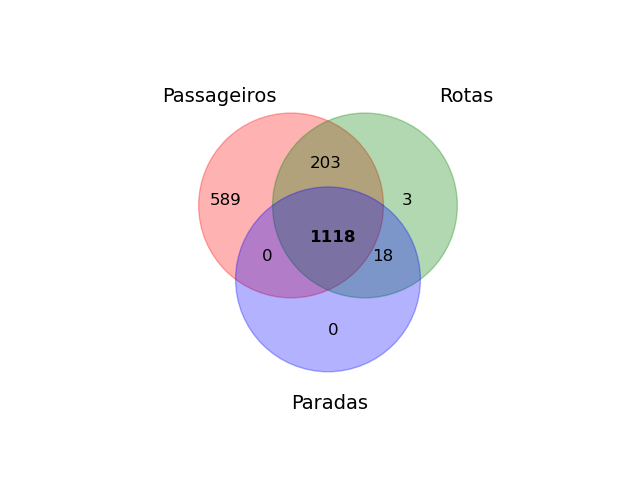
\includegraphics[width=0.8\textwidth]{figuras/diagrama_de_venn_intersec_rotas_passageiros_paradas.png}
    \caption{Diagrama de Venn com as intersecções de rotas entre as bases passageiros, paradas e rotas \\ Fonte: A própria autora}
    \label{fig:minha-imagem}
\end{figure}

Com o diagrama, conseguimos visualizar que 1118 linhas aparecem nas 3 tabelas (passageiros, rotas e paradas), 589 aparecem apenas em passageiros e 3 aparecem apenas em rotas, 203 aparecem em passageiros e rotas (não possuem paradas) e 18 aparecem em rotas e paradas (não possuem dados de passageiros). Assim, podemos analisar de modo mais aprofundado cada um desses casos.

\subsubsection{Rotas descontinuadas}

Foram identificadas um total de \textbf{589 rotas} que estão na base de passageiros, mas não estão na base de rotas. Abaixo, apresentamos uma tabela detalhada com o número de passageiros transportados e a quantidade de dias em que temos dados das linhas:
% tabela 

\begingroup
\small % reduz o tamanho da fonte da tabela

\sisetup{
  round-precision = 1,
  table-number-alignment = left,
  table-format = 3.1, % até milhar com uma casa decimal
}

\begin{longtable}[c]{
  l
  l
  l
  l
  l
}


\toprule
{Período} &
\makecell{101--1.000\\passageiros} &
\makecell{1001--10.000\\passageiros} &
\makecell{$\leq$100\\passageiros} &
\makecell{$>$10.000\\passageiros} \\
\midrule
\endfirsthead

\toprule
{Período} &
\makecell{101--1.000\\passageiros} &
\makecell{1001--10.000\\passageiros} &
\makecell{$\leq$100\\passageiros} &
\makecell{$>$10.000\\passageiros} \\
\midrule
\endhead

\multicolumn{5}{r}{\textit{continua}\enspace$\longrightarrow$} \\
\caption[]{Distribuição de passageiros por período.}
\endfoot

\bottomrule
\caption[]{Distribuição de passageiros por período. Fonte: A própria autora}
\endlastfoot

\captionlistentry{Distribuição de passageiros por período.}\label{tab:distribuicao-passageiros}

30--90 dias  & 0.0 & 0.0 & 0.0 & 72.0 \\
91--365 dias & 0.0 & 0.0 & 0.0 & 65.0 \\
$\leq$30 dias & 3.0 & 12.0 & 2.0 & 176.0 \\
$>$365 dias   & 0.0 & 0.0  & 0.0 & 197.0 \\

\end{longtable}
\endgroup


Com base nessas estatísticas, podemos afirmar que a maioria dos dados sobre linhas que estão na tabela de passageiros, mas não estão na tabela de rotas são ou de linhas que operaram durante muito tempo e transportaram muitos passageiros (33,44\%) ou que operaram durante menos de um mês e transportaram muitos passageiros (29,88\%). Concluímos, então, que é crucial analisar essas rotas faltantes, que foram extintas ou modificadas, para analisar a eficiência do transporte, já que um grande número de passageiros foi impactado por essas mudanças.



\subsubsection{Rotas sem paradas}

Há 203 rotas cadastradas sem informações sobre  paradas. Sem esses dados, não é possível realizar análises geográficas. Ao examinar quais rotas são afetadas, identificamos, por exemplo, a linha 177H-10 (Cidade Universitária – Metrô Santana), que de fato não aparece na tabela de viagens. No entanto, observamos que há registros para a linha 177H-21, que opera aos sábados e percorre um trajeto semelhante.

A partir da análise da rota 177H, notamos que, ao considerar apenas os quatro primeiros caracteres do código da linha, o número de rotas sem paradas cai de 203 para 47. Apesar disso, utilizar essa aproximação introduz possíveis inconsistências, pois os dois últimos dígitos do código da linha são essenciais para distinguir rotas diferentes. Por exemplo, a linha 778J-10 faz o trajeto Jardim Arpoador – Metrô Barra Funda, enquanto a 778J-41 percorre Cohab Raposo Tavares – Metrô Barra Funda. Apesar de ambas passarem por trechos semelhantes e compartilharem destino final, tratam-se de rotas distintas. 

Entre essas 47 linhas restantes, destacam-se as que circulam pela Cidade Universitária (8082-10, 8083-10, 8084-10 e 8085-10), além de outras de conhecimento da autora, como a 7725-10 (Lapa – Rio Pequeno), que também passa pela cidade universitária, e a 8021-10 (Jardim Maria Luiza – Butantã). A ausência de dados completos no GTFS inviabiliza qualquer análise dessas linhas. Portanto, possívelmente, há um problema de ingestão dos dados por parte das empresas que operam as linhas, que possívelmente não cadastraram todos os dados necessários para a operação de cada linha.

Essa lacuna representa uma falha de transparência e cuidado na disponibilização de dados sobre o transporte público na maior metrópole da América Latina, onde mais de 20 milhões de pessoas circulam diariamente. Para cobrir essa lacuna, solicitamos a SPTrans o envio dos dados históricos do GTFS, que será tratada na seção \ref{sec:esic}.

\subsubsection{Rotas sem passageiros}

Notamos que todas as rotas que não possuem dados de passageiros, mas possuem dados de paradas, são, na verdade, erros de digitação. Todas estão duplicadas na tabela de rotas, como o exemplo abaixo:

\begin{table}
\centering
\begin{tabular}{ll}
\toprule
 route\_id &                        route\_long\_name \\
\midrule
909T1 & Term. Pinheiros - Term. Pq. D. Pedro Ii \\
909T10 & Term. Pinheiros - Term. Pq. D. Pedro Ii \\
\bottomrule
\end{tabular}
\caption{Rotas sem passageiros. Fonte: A própria autora}
\end{table}

Desse modo, vamos desconsiderar esses dados ausentes.

\subsubsection{Rotas sem passageiros e paradas}

Há apenas 3 rotas sem passageiros e paradas, sendo uma delas o Circular Turismo. Podemos notar que também parece haver erro de digitação no id das rotas, já que todas as que operam na cidade possuem 6 dígitos. Também vamos desconsiderar essa ausência de dados.

\begin{table}
\centering
\begin{tabular}{llll}
\toprule
 route\_id & route\_short\_name &                          route\_long\_name \\
\midrule
    83001 &           8300-1 &              Term. Pirituba - Term. Lapa \\
    909T1 &           909T-1 &  Term. Pinheiros - Term. Pq. D. Pedro Ii \\
    CT011 &           CT01-1 &                       Circular - Turismo \\
\bottomrule
\end{tabular}
\caption{Rotas sem passageiros e paradas. Fonte: A própria autora}
\end{table}

\section{Solicitação de dados ao Serviço de Informação ao Cidadão}
\label{sec:esic}

A partir da identificação de 589 rotas descontinuadas e 206 rotas sem dados de paradas, criamos uma solicitação ao Serviço de Informação ao Cidadão por meio eletrônico (SIC-e) para recebermos o histórico de dados do GTFS de janeiro de 2015 a março de 2025, o qual possui prazo para ser processado  de até 20 (vinte) dias, estabelecido no § 2º do art. 18 do Decreto Municipal 53.623/2012. Obtivemos resposta após 18 dias corridos da solicitação.

Recebemos, da SPTrans, o acesso aos dados solicitados por meio do Google Drive, com arquivos mensais, tendo os dados do GTFS de janeiro de 2015 a março de 2025, sendo cada arquivo no mesmo formato daquele disponibilizado na seção para desenvolvedores da SPTrans. Além disso, a empresa demonstrou interesse em conhecer o trabalho acadêmico desenvolvido e indicou o contato do responsável pela Gerência de Avaliação de Transporte e Experiência do Usuário, para eventual compartilhamento dos resultados.

A partir dos dados enviados, buscamos construir uma base histórica do GTFS que permita, para qualquer data específica, associar as informações de uma determinada linha aos passageiros que a utilizaram.

Como a solicitação dos dados ao SIC-e teve origem em inconsistências previamente identificadas, nosso objetivo agora é avaliar se essas inconsistências persistem.

\subsection{Análise das inconsistências}

Ao replicar a mesma análise que fizemos na seção \ref{sec:exploracaoinicial}, verificamos que a maior parte dos registros (1.570) está presente simultaneamente nas três bases (passageiros, rotas e paradas). Isso representa um aumento de 40\% na intersecção entre elas, indicando uma boa integração e maior consistência dos dados.

\begin{figure}[H]
    \centering
    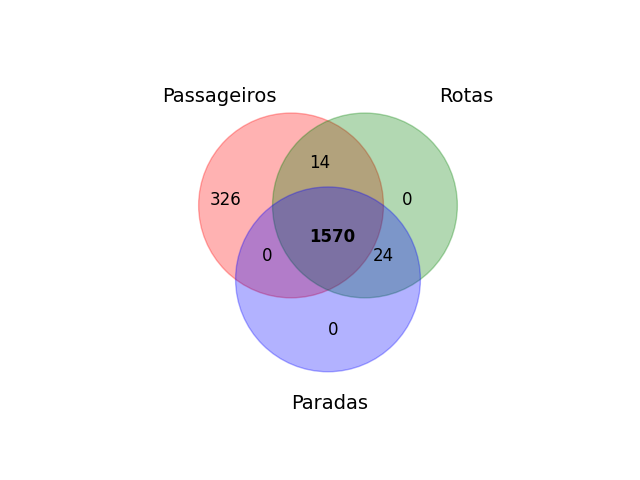
\includegraphics[width=0.8\textwidth]{figuras/diagrama_de_venn_intersec_rotas_passageiros_paradas_historico.png}
    \caption{Diagrama de Venn com as intersecções de rotas entre as bases passageiros, paradas e rotas \\ Fonte: A própria autora}
    \label{fig:minha-imagem}
\end{figure}

Ainda assim, a base de passageiros contém 326 linhas que não aparecem nas bases de rotas ou paradas. Embora esse número seja menor que os 589 registros identificados anteriormente, ele ainda sugere a presença de dados incompletos. Além disso, há interseções parciais de menor relevância: 14 registros aparecem apenas entre passageiros e rotas, e 24 entre rotas e paradas. Vale destacar que não há linhas exclusivas das tabelas de rotas ou paradas, nem linhas que apareçam apenas nas bases de passageiros e paradas.

Das 589 linhas que anteriormente não haviam sido identificadas na tabela de passageiros e que não aparecem na tabela de rotas ou paradas, 326 continuam sem dados associados. Ao analisarmos o período de operação dessas linhas, verificamos que a maioria se refere a linhas temporárias, que funcionaram por menos de um mês. Apesar do curto período de atividade, essas rotas transportaram um número relevante de passageiros e, provavelmente, foram posteriormente substituídas por linhas permanentes ou reconfiguradas dentro do sistema de transporte, aparecendo no GTFS com outro nome. 



\begin{table}[htbp]
\centering
\resizebox{\textwidth}{!}{%
\begin{tabular}{lrrrr}
\toprule
passageiros &  1001-10000 passageiros &  101-1.000 passageiros &  <=100 passageiros &  >10.000 \\
periodo     &                         &                        &                    &          \\
\midrule
30-90 dias  &                     0.0 &                    0.0 &                0.0 &     20.0 \\
91-365 dias &                     0.0 &                    0.0 &                0.0 &     10.0 \\
<=30 dias   &                    10.0 &                    2.0 &                2.0 &    164.0 \\
>365        &                     0.0 &                    0.0 &                0.0 &     56.0 \\
\bottomrule
\end{tabular}
}
\caption{Quantidade de passageiros por tempo de operação das linhas. Fonte: A própria autora}
\label{tab:distancias_rotas}
\end{table}

Quanto as outras 14 linhas que possuem dados de paradas mas não de passageiros, vamos desconsiderar da análise. Já nas linhas que possuem dados de passageiros e rotas, mas não de paradas, observamos uma diminuição da inconsistência de mais de 93\%, sobrando apenas 14 linhas das 203 levantadas anteriormente. 

Como já possuímos o histórico completo do GTFS fornecido pela SPTrans, vamos descartar os registros com as inconsistências mencionadas nessa seção.

\section{Descrição da estrutura final dos dados}

\subsection{Rotas}

A tabela de rotas contém informações sobre as linhas de ônibus operantes no município de São Paulo ao longo do período de janeiro de 2015 a março de 2025. Possui 167.346 registros distribuídos em 8 colunas, contendo atributos como o identificador da rota ($route\_id$), identificador da agência ($agency\_id$), nome curto e nome completo da linha ($route\_short\_name, route\_long\_name$), tipo de rota ($route\_type$), além de dados de cores utilizadas ($route\_color$ e $route\_text\_color$). 

A coluna $data\_referencia$ indica o mês e ano onde a rota existiu no GTFS. Notamos que as colunas de cores apresentam valores ausentes em datas mais antigas, sendo esse um valor preenchido apenas nos dados mais recentes.

\subsection{Paradas}
A tabela de paradas de ônibus possui informações detalhadas sobre cada parada realizada pelas viagens das rotas, entre janeiro de 2015 e março de 2025. Com 11.849.701 registros e 13 colunas, seu tamanho total ultrapassa 1 GB.

Os dados incluem identificadores de rota ($route\_id$), viagem ($trip\_id$), serviço ($service\_id$), direção da viagem ($direction\_id$) e sequência da parada ($stop\_sequence$), além de informações textuais como o nome e a descrição da parada ($stop\_name, stop\_desc$). Também estão presentes as coordenadas geográficas ($stop\_lat, stop\_lon$). A coluna $data\_referencia$ indica o mês e ano onde a parada existiu no GTFS.

\subsection{Passageiros}

A tabela correspondente ao histórico de passageiros transportados fornece uma visão detalhada da demanda por linha de ônibus ao longo do tempo, abrangendo o período de 1 de janeiro de 2015 a 07 de setembro de 2025. Com um total de 5.056.912 registros distribuídos em 25 colunas, seu volume de dados ultrapassa 1 GB.

As colunas registram, para cada linha e data específica, a quantidade de passageiros segmentada por tipo de pagamento e perfil do usuário, como $passageiros\_dinheiro$, $passageiros\_comum$, $passageiros\_vale_transporte$, $passageiros\_estudante$ e $passageiros\_gratuitos$, entre outras. Além disso, há colunas de totalizações como $passageiros\_pagantes$, $passageiros\_total$ e $passageiros\_integracao$, permitindo a análise de diferentes perfis de uso do transporte público. As variáveis $empresa$, $linha$, $area$, $grupo$, $lote$ e $route\_id$ fornecem informações complementares sobre a operação do sistema e sua organização espacial e institucional. A coluna $data$ representa a data para a qual o registro de passageiros de uma respectiva linha se refere, com granularidade diária.

\subsection{População}

A base de dados referente à população por bairro, obtida a partir do Censo Demográfico de 2022 do IBGE, contém 17.576 registros e 27 colunas, organizadas como um GeoDataFrame da biblioteca GeoPandas, o que possibilita a realização de análises espaciais. A tabela inclui identificadores e nomes de diversas divisões administrativas, como região, município, distrito, subdistrito, bairro, e região integrada, bem como a área territorial ($AREA\_KM2$) e a geometria espacial correspondente a cada unidade territorial. As colunas de $v0001$ a $v0007$ representam indicadores populacionais e domiciliares, conforme o dicionário de variáveis disponibilizado pelo IBGE na tabela \ref{tab:variaveis_domicilios_populacao}.

Para complementar esses dados, temos a subdivisão em zonas, onde, para cada distrito, atribuimos uma das 5 zonas: Norte, Sul, Leste, Oeste e Centro. Essa base possui 3 colunas (Regiões, Subprefeituras e Distritos) e 96 registros.

\subsection{Estações de trem e metrô}

A base de estações de trem e metrô conta com o nome da estação, o nome linha e a localização geográfica (em formato de geometria) da estação, além da indicação de estação planejada ou existente.

\subsection{Merges}

Nas tabelas de rotas, passageiros e paradas, as colunas-chave para realizar a junção das tabelas principais são $route\_id$ e $data$ (ou $data\_referencia$), utilizadas para associar, ao longo do tempo, os dados das rotas, paradas e passageiros transportados. A partir dessas colunas, foi possível consolidar uma estrutura temporal da operação do transporte público.

Para o restante dos dados, a base de paradas foi definida como estrutura central da modelagem, uma vez que cada registro representa um ponto geográfico ao longo do sistema de transporte. A ela foram adicionadas as demais bases por meio de junções espaciais, utilizando as coordenadas geográficas disponíveis na coluna $geometry$, principalmente por um join espacial de proximidade, conforme explicado nas respectivas seções dessas bases (\ref{sec:ibge} e \ref{sec:trem_metro}).

Essa estrutura unificada, centralizada nas paradas de ônibus, permite uma análise integrada entre demanda por transporte, localização, acesso à rede metrô-CPTM e características populacionais.

\begin{figure}[h]
    \centering
    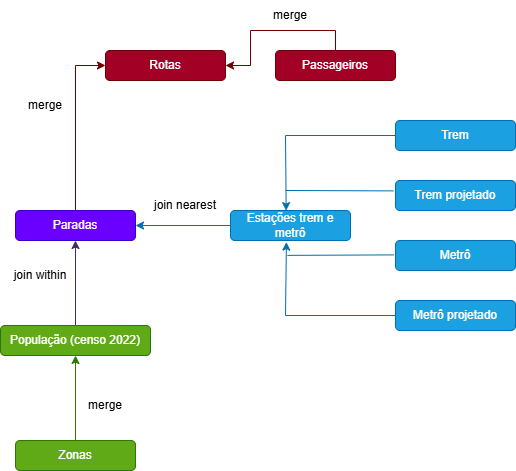
\includegraphics[width=0.8\textwidth]{figuras/schema tabelas relações.drawio.png}
    \caption{Diagrama com as tabelas do trabalho e suas relações \\ Fonte: A própria autora}
    \label{fig:minha-imagem}
\end{figure}

\section{Grafos}

Nesta seção, vamos abordar o que é um grafo, por que essa estrutura é importante para nossa análise e como criar e analisar ela com os dados obtidos no trabalho.

\subsection{Definição}

Um grafo é uma estrutura usada para representar relações entre objetos, formado por um conjunto de vértices (ou nós) e um conjunto de arcos (ou arestas). Cada aresta liga dois nós, indicando uma conexão ou relação entre eles. Podemos imaginar um grafo como um mapa de transporte: os nós seriam as estações (ou paradas) e as arestas, as linhas que ligam as estações e formam uma rota, em mão única. Por exemplo, se há um arco que vai do vértice A para o vértice B, isso significa que há um caminho que sai de A e chega em B. Visualmente, podemos observar um grafo no próprio mapa da rede de trem e metrô de São Paulo:

\begin{figure}[H]
    \centering
    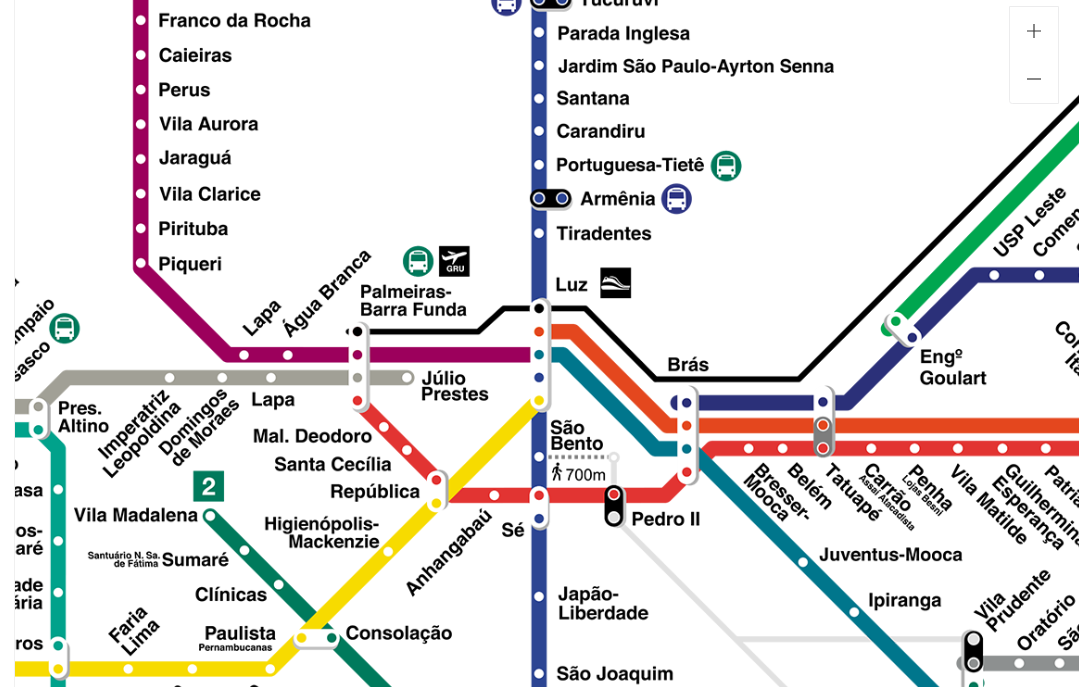
\includegraphics[width=0.8\textwidth]{figuras/mapa metro.png}
    \caption{Mapa do metrô de São Paulo \\ Fonte: Companhia Paulista de Trens Metropolitanos (CPTM)}
    \label{fig:minha-imagem}
\end{figure}

\subsection{Aplicação}

Para modelar a rede de transporte público por ônibus da cidade de São Paulo, \citet{tcc:Danilo} construiu, a partir dos dados provenientes do Bilhete Único, grafos não orientados, cujos vértices representam regiões político-administrativas da cidade e as arestas indicam as conexões viárias estabelecidas por linhas de ônibus entre essas regiões. O foco da análise foi em identificar o volume de passageiros nos horários de pico,  permitindo identificar os principais fluxos de deslocamento nos períodos de maior demanda. Essa modelagem permitiu a visualização das áreas mais saturadas do sistema e forneceu subsídios para análises sobre a eficiência e a cobertura do transporte público, evidenciando a aplicabilidade dos grafos na compreensão e no planejamento urbano.

De modo semelhante, vamos criar um grafo com os dados do GTFS para analisar algumas métricas de centralidade. O grafo será criado utilizando as paradas como nós, e as viagens como arestas. Como não conseguimos fazer os joins que queriamos para saber a população afetada diretamente por uma parada, vamos fazer análises mais simples, focando em métricas de centralidade do grafo.

\subsubsection{Como criar o grafo}

A Peartree é uma biblioteca feita em Python, projetada para criar grafos a partir de dados GTFS. Ela permite transformar informações sobre paradas, rotas e horários em um grafo geoespacial, facilitando análises como cálculo de rotas, centralidade de estações e conectividade da rede. 

Embora a Peartree não esteja mais sendo atualizada e tenha limitações em relação a algumas funcionalidades como a integração de dados complementares de passageiros, optamos por utilizá-la devido à sua facilidade de uso e integração direta com os dados GTFS. A partir de um caminho de arquivo .zip no formato GTFS, um horário de início e um horário final, a peartree devolve um objeto de grafo da biblioteca Networkx, que permite diversas análises com métodos já implementados.

Para o nosso trabalho, vamos criar um grafo para cada mês de dados do GTFS, com o objetivo de obter dados temporais para algumas métricas. Como o sistema é muito pesado, optamos por criar um grafo com as rotas que operam entre 06h e 08h, pegando o horário de pico da manhã. Vale notar que, mesmo com essa limitação de horário, a criação de todos os grafos e o cálculo de algumas métricas de centralidade levou cerca de 8h para executar.

\subsubsection{Cálculo de métricas de centralidade}

Para quantificar a importância de um nó, podemos calcular algumas métricas de centralidade, que foram melhor definidas e estudadas por \citet{FREEMAN1978215}, sendo elas: Centralidade de Grau (Degree Centrality), Centralidade de Proximidade (Closeness Centrality) e Centralidade de Intermediação (Betweenness Centrality).

A Centralidade de Grau (Degree Centrality) é calculada simplesmente pela contagem do número de arestas que um nó possui. Essa medida permite avaliarmos quão importante um nó é para a rede. No nosso caso, por exemplo, nós com alta centralidade possívelmente estarão localizados em vias importantes, por onde passam várias linhas, como a Av. Paulista, Av. Rebouças, e etc.

\begin{equation*}
C_D(v) = \frac{k_v}{N - 1}
\end{equation*}

onde:
\begin{itemize}
    \item $C_D(v)$ é a Centralidade de Grau do nó $v$;
    \item $k_v$ é o grau do nó $v$ (número de conexões);
    \item $N$ é o número total de nós na rede.
\end{itemize}

A Centralidade de Proximidade (Closeness Centrality) avalia a importância de um nó em um contexto global, baseada no conceito de distância, sendo o inverso da soma das distâncias geodésicas (os caminhos mais curtos) de um nó a todos os outros. Nós com alta proximidade são aqueles que permitem a um passageiro chegar em outro lugar mais facilmente, pois possuem a menor distância média para alcançar o restante dos nós.

\begin{equation*}
C_C(v) = \frac{N - 1}{\sum_{u \neq v} d(v, u)}
\end{equation*}

onde:
\begin{itemize}
    \item $C_C(v)$ é a Centralidade de Proximidade do nó $v$;
    \item $N$ é o número total de nós na rede;
    \item $d(v, u)$ é a distância (caminho mais curto) entre $v$ e $u$.
\end{itemize}

A Centralidade de Intermediação (Betweenness Centrality) avalia o quanto um nó atua como "ponte" ou "intermediário" nos caminhos mais curtos entre outros pares de nós, ocupando uma posição estratégica na rede. No nosso grafo, podemos esperar que os nós em vias importantes também tenham uma alta betweenness centrality.

\begin{equation*}
C_B(v) = \sum_{s \neq v \neq t} \frac{\sigma_{st}(v)}{\sigma_{st}}
\end{equation*}

onde:
\begin{itemize}
    \item $C_B(v)$ é a Centralidade de Intermediação do nó $v$;
    \item $\sigma_{st}$ é o número total de caminhos mais curtos entre $s$ e $t$;
    \item $\sigma_{st}(v)$ é o número desses caminhos que passam pelo nó $v$.
\end{itemize}

\section{Cálculo da distância percorrida pelas rotas}

Para calcular a distância percorrida por uma rota, utilizamos duas abordagens: primeiro, vamos somar a distância percorrida entre cada parada da rota, seguindo a sequência de paradas de cada viagem da rota, para saber qual o seu percurso real. Segundo, vamos calcular qual a distância máxima entre duas paradas de uma rota, para saber qual a distância que ela percorre pela cidade. Faremos isso para cada mês entre 2015 e março de 2025, para obteros uma sequência cronológica dessas distâncias.

Para obter uma medida mais realista de proximidade entre paradas, utilizamos a distância geográfica real entre coordenadas (latitude e longitude), em vez da distância topológica (número de arestas). Essa abordagem transforma o grafo em uma estrutura espacialmente ponderada, em que cada aresta tem um peso correspondente à distância em metros entre paradas consecutivas, sendo amplamente usada em redes urbanas reais, como discutido por \citep{barthelemy2011spatial}, que destaca a importância de considerar as dimensões geográficas nas análises de conectividade. \citet{rodrigue2020geography} também reforça que sistemas de transporte público devem ser modelados como redes geoespaciais, onde a posição das paradas influencia diretamente a eficiência do transporte.

A distância geográfica entre duas paradas $d(u,v)$ é calculada utilizando a fórmula de Haversine, que considera o raio da Terra para estimar a menor distância ao longo da superfície esférica. 

\begin{equation}
d(p, q) = 2R \cdot \arcsin\left( \sqrt{ \sin^2\left( \frac{\Delta \phi}{2} \right) + \cos(\phi_1) \cos(\phi_2) \sin^2\left( \frac{\Delta \lambda}{2} \right) } \right)
\end{equation}

\noindent
Onde:
\begin{itemize}
  \item \( d \): distância entre os dois pontos, em metros;
  \item \( R \): raio médio da Terra, aproximadamente \( 6.371 \) quilômetros;
  \item \( \phi_1, \phi_2 \): latitudes dos pontos 1 e 2 (em radianos);
  \item \( \lambda_1, \lambda_2 \): longitudes dos pontos 1 e 2 (em radianos);
  \item \( \Delta \phi = \phi_2 - \phi_1 \): diferença de latitude;
  \item \( \Delta \lambda = \lambda_2 - \lambda_1 \): diferença de longitude.
\end{itemize}

Para implementar esses métodos em Python, utilizamos as bibliotecas math, scipy e numpy, além da função geodesic do módulo distance do geopy.


\section{Noções estatísticas}

Para entender os resultados do trabalho, vamos abordar o conceito de regressão linear e o que é e como interpretar um boxplot.

\subsection{Regressão linear}

A regressão linear é um dos modelos estatísticos mais utilizados para descrever a relação entre duas variáveis. Tendo em vista que não temos a população inteira, o modelo sempre será acompanho de erros (resíduos), os quais usaremos para quantificar quão boa é nossa hipótese de que as variáveis possuem uma dependência linear. O modelo pode ser calculado por 
\begin{equation*}
\hat{y}_i = \hat{\alpha} + \hat{\beta}\times\hat{x}_{i},
\end{equation*} sendo os valores de $\hat{\alpha}$ e $\hat{\beta}$ calculados pelo método dos mínimos quadrados. Os resíduos do modelo podem ser calculados por 
\begin{equation*}
\hat{e}_i = y_i - \hat{y}_{i},
\end{equation*} e possuem média zero, variância constante (homocedasticidade), independência entre si e distribuição normal \citep{MorettinSinger2019}. Com essas características, podemos calcular, a partir desses resíduos, quão estatísticamente significativo é o modelo de regressão linear para os dados. Um p-valor baixo indica que a hipótese de que não há relação linear entre as variáveis é falsa, mas não implica, necessariamente, que essa relação é verdadeira \citep{pvalue}. Outra métrica que podemos avaliar é o $R^2$, que indica quanto da variação dos dados é explicada pelo modelo, sendo calculada como a diferença entre 1 e a razão entre a soma dos quadrados dos resíduos e a soma do quadrado dos dados \citep{MorettinSinger2019}. Para a implementação desses estudos neste trabalho, usamos o módulo $linregress$ da biblioteca de Python $scipy.stats$ e, para identificar a normalidade dos resíduos, utilizamos o QQ Plot, um gráfico que compara os resíduos da regressão com a distribuição normal teórica. Se os pontos estiverem próximos da linha diagonal, os resíduos seguem aproximadamente uma distribuição normal, grandes desvios indicam não normalidade.

\subsection{O boxplot}

O boxplot, introduzido por \citet{tukey1977exploratory} permite visualizar a distribuição de um conjunto de dados e identificar valores atípicos. Ela resume os principais atributos dos dados através de 5 estatísticas principais: o mínimo, o máximo, a mediana, o primeiro quartil e o terceiro quartil.

\begin{figure}[H]
    \centering
    {%
        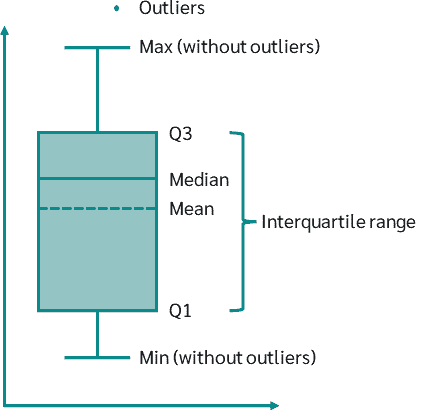
\includegraphics[width=0.6\textwidth]{figuras/boxplot-interpretation.png}
    }
    \caption{Ilustração dos atributos de um boxplot. Fonte: Numiqo.}
\end{figure}

Neste trabalho, utilizaremos o boxplot para visualizar a distribuição de métricas dos dados, de forma a não nos prendermos apenas na média ou mediana, principalmente quando considerarmos o alto volume de 10 anos de dados.

